\section{Experimental Simulation Results}
\label{sec:experimentation}
The simulation model involved creating a test environment that could be run without user interaction. To accomplish the simulation a web-application was built using Java as the programming language and \href{https://spring.io/projects/spring-boot}{Spring Boot} as the dependency injection framework. An in-memory H2 database solution was used in order to simulate data transactions within the application as well. Once the application was built, it was containerized into a \href{https://www.docker.com/}{Docker} container and deployed on cloud computing resources using \href{https://www.digitalocean.com/}{Digital Ocean} as the computing power. The simulation ran many hours generating thousands of results that were uploaded into an \href{https://aws.amazon.com/s3/}{Amazon S3 bucket} for retrieval. The results were pulled and analyzed using \href{https://www.tableau.com/}{Tableau} to discover the patterns and trends within the data. The experimentation setup involved running 3 solutions (the 2PL solution, the no-locking solution, and the prediction-based solution) with varying workloads through 7 different test cases (Table \ref{tbl:sim_test_cases} outlines the seven test cases developed according to the percentage of each transaction category [Definition \ref{transaction_categories}]). These test cases ensured that a wide range of testing workloads were covered in all categorization scenarios. To simulate the overhead of compensation transactions in comparison to the prediction-based scheduler we used the SAGA implementation pattern to calculate the additional execution time \cite{SAGAS-Garcaa-Molrna}. This pattern is built by using equal and opposite actions to each operation in a business process to revert the changes of an operation that fails. This metric allows us to simulate the overhead of a compensation transaction for each transaction that fails.

%%%%Start writing here with analysis of results
In analyzing the results, we generated 14 different plots (two for each test case). The plots visualize all executions across all three solutions in comparison to the workload. In each graph, there are three lines representing the comparison between the solutions. There are three levels of line thickness for each of the execution times increasing in the order of no-locking execution time, traditional 2PL execution time, and prediction-based execution time. The graphs appear to show only two lines due to the prediction-based solution and the traditional solutions execution time being so close. Figures \ref{results:consistency_test_case_graphs_1_4} \& \ref{results:consistency_test_case_graphs_5_7} are another view of the same data showing the comparison of the prediction-based solution against the 2PL and the no-locking solution when consistency is lost and retained. In all cases, we see the execution time increase when consistency is lost in the no-locking solution (top graph), and execution time remains comparable to the 2PL solution when consistency is kept by the prediction-based solution (bottom graph).

In all test cases, we see that consistency was retained in both the 2PL solution and the prediction-based solution, but when the no-locking solution loses consistency, the efficiency decreases due to the compensation transaction. Our empirical results confirm that the performance of our prediction-based solution performs to the traditional 2PL locking solution with the added benefit of deadlock avoidance due to the lock action (see Definition \ref{legal_scheduler}) within the prediction-based solution.

\begin{table}[h]
\captionsetup{justification=centering}
\centering
\begin{tabular}{|c|c|c|c|c|}
\hline
\multicolumn{5}{|c|}{\cellcolor[HTML]{EFEFEF}\textbf{Simulation Test Cases}}                                                   \\ \hline
\textbf{Test Case \#} & \textbf{HCHE} & \textbf{HCLE} & \textbf{LCHE} & \textbf{LCLE} \\ \hline
1 & 100\% & 0\% & 0\% & 0\% \\ \hline
2 & 75\% & 25\% & 0\% & 0\% \\ \hline
3 & 50\% & 25\% & 25\% & 0\% \\ \hline
4 & 25\% & 25\% & 25\% & 25\% \\ \hline
5 & 0\% & 25\% & 25\% & 50\% \\ \hline
6 & 0\% & 0\% & 25\% & 75\% \\ \hline
7 & 0\% & 0\% & 0\% & 100\% \\ \hline
\end{tabular}

\caption{Simulation Test Cases} % title of the Figure
\label{tbl:sim_test_cases} % label to refer figure in text

\end{table}

\begin{figure}
\centering
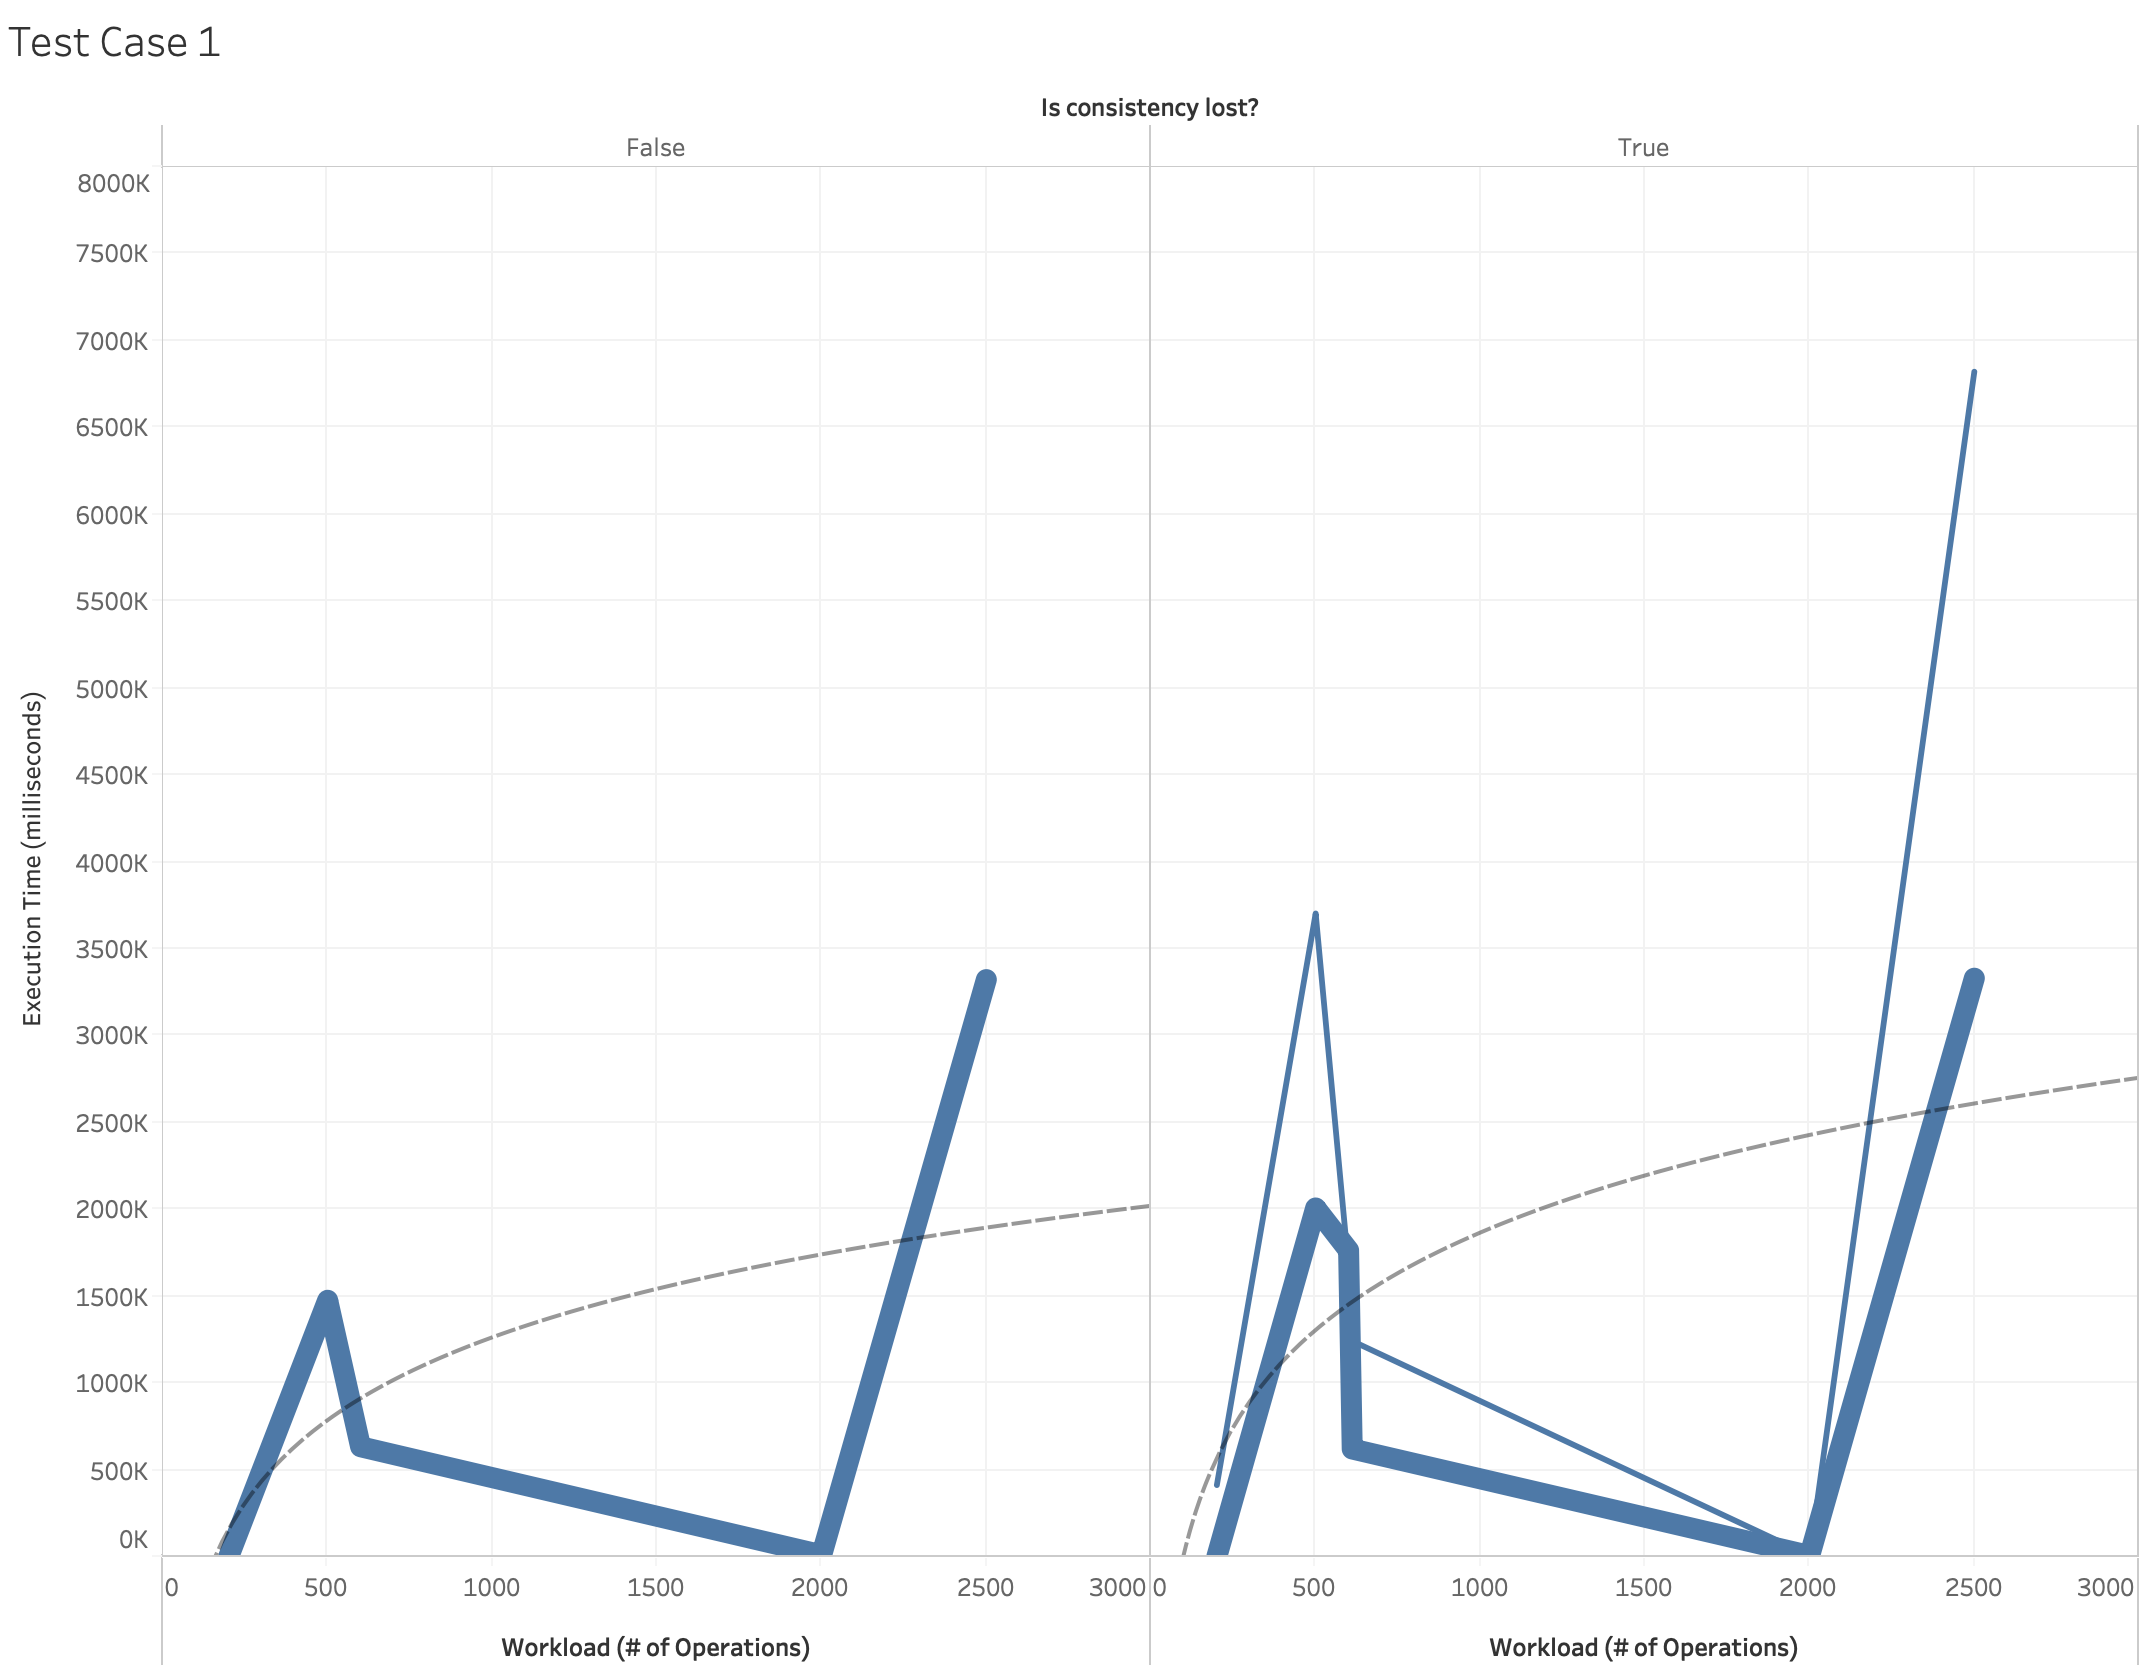
\includegraphics[scale=0.11]{images/TestCase1(WL).png}
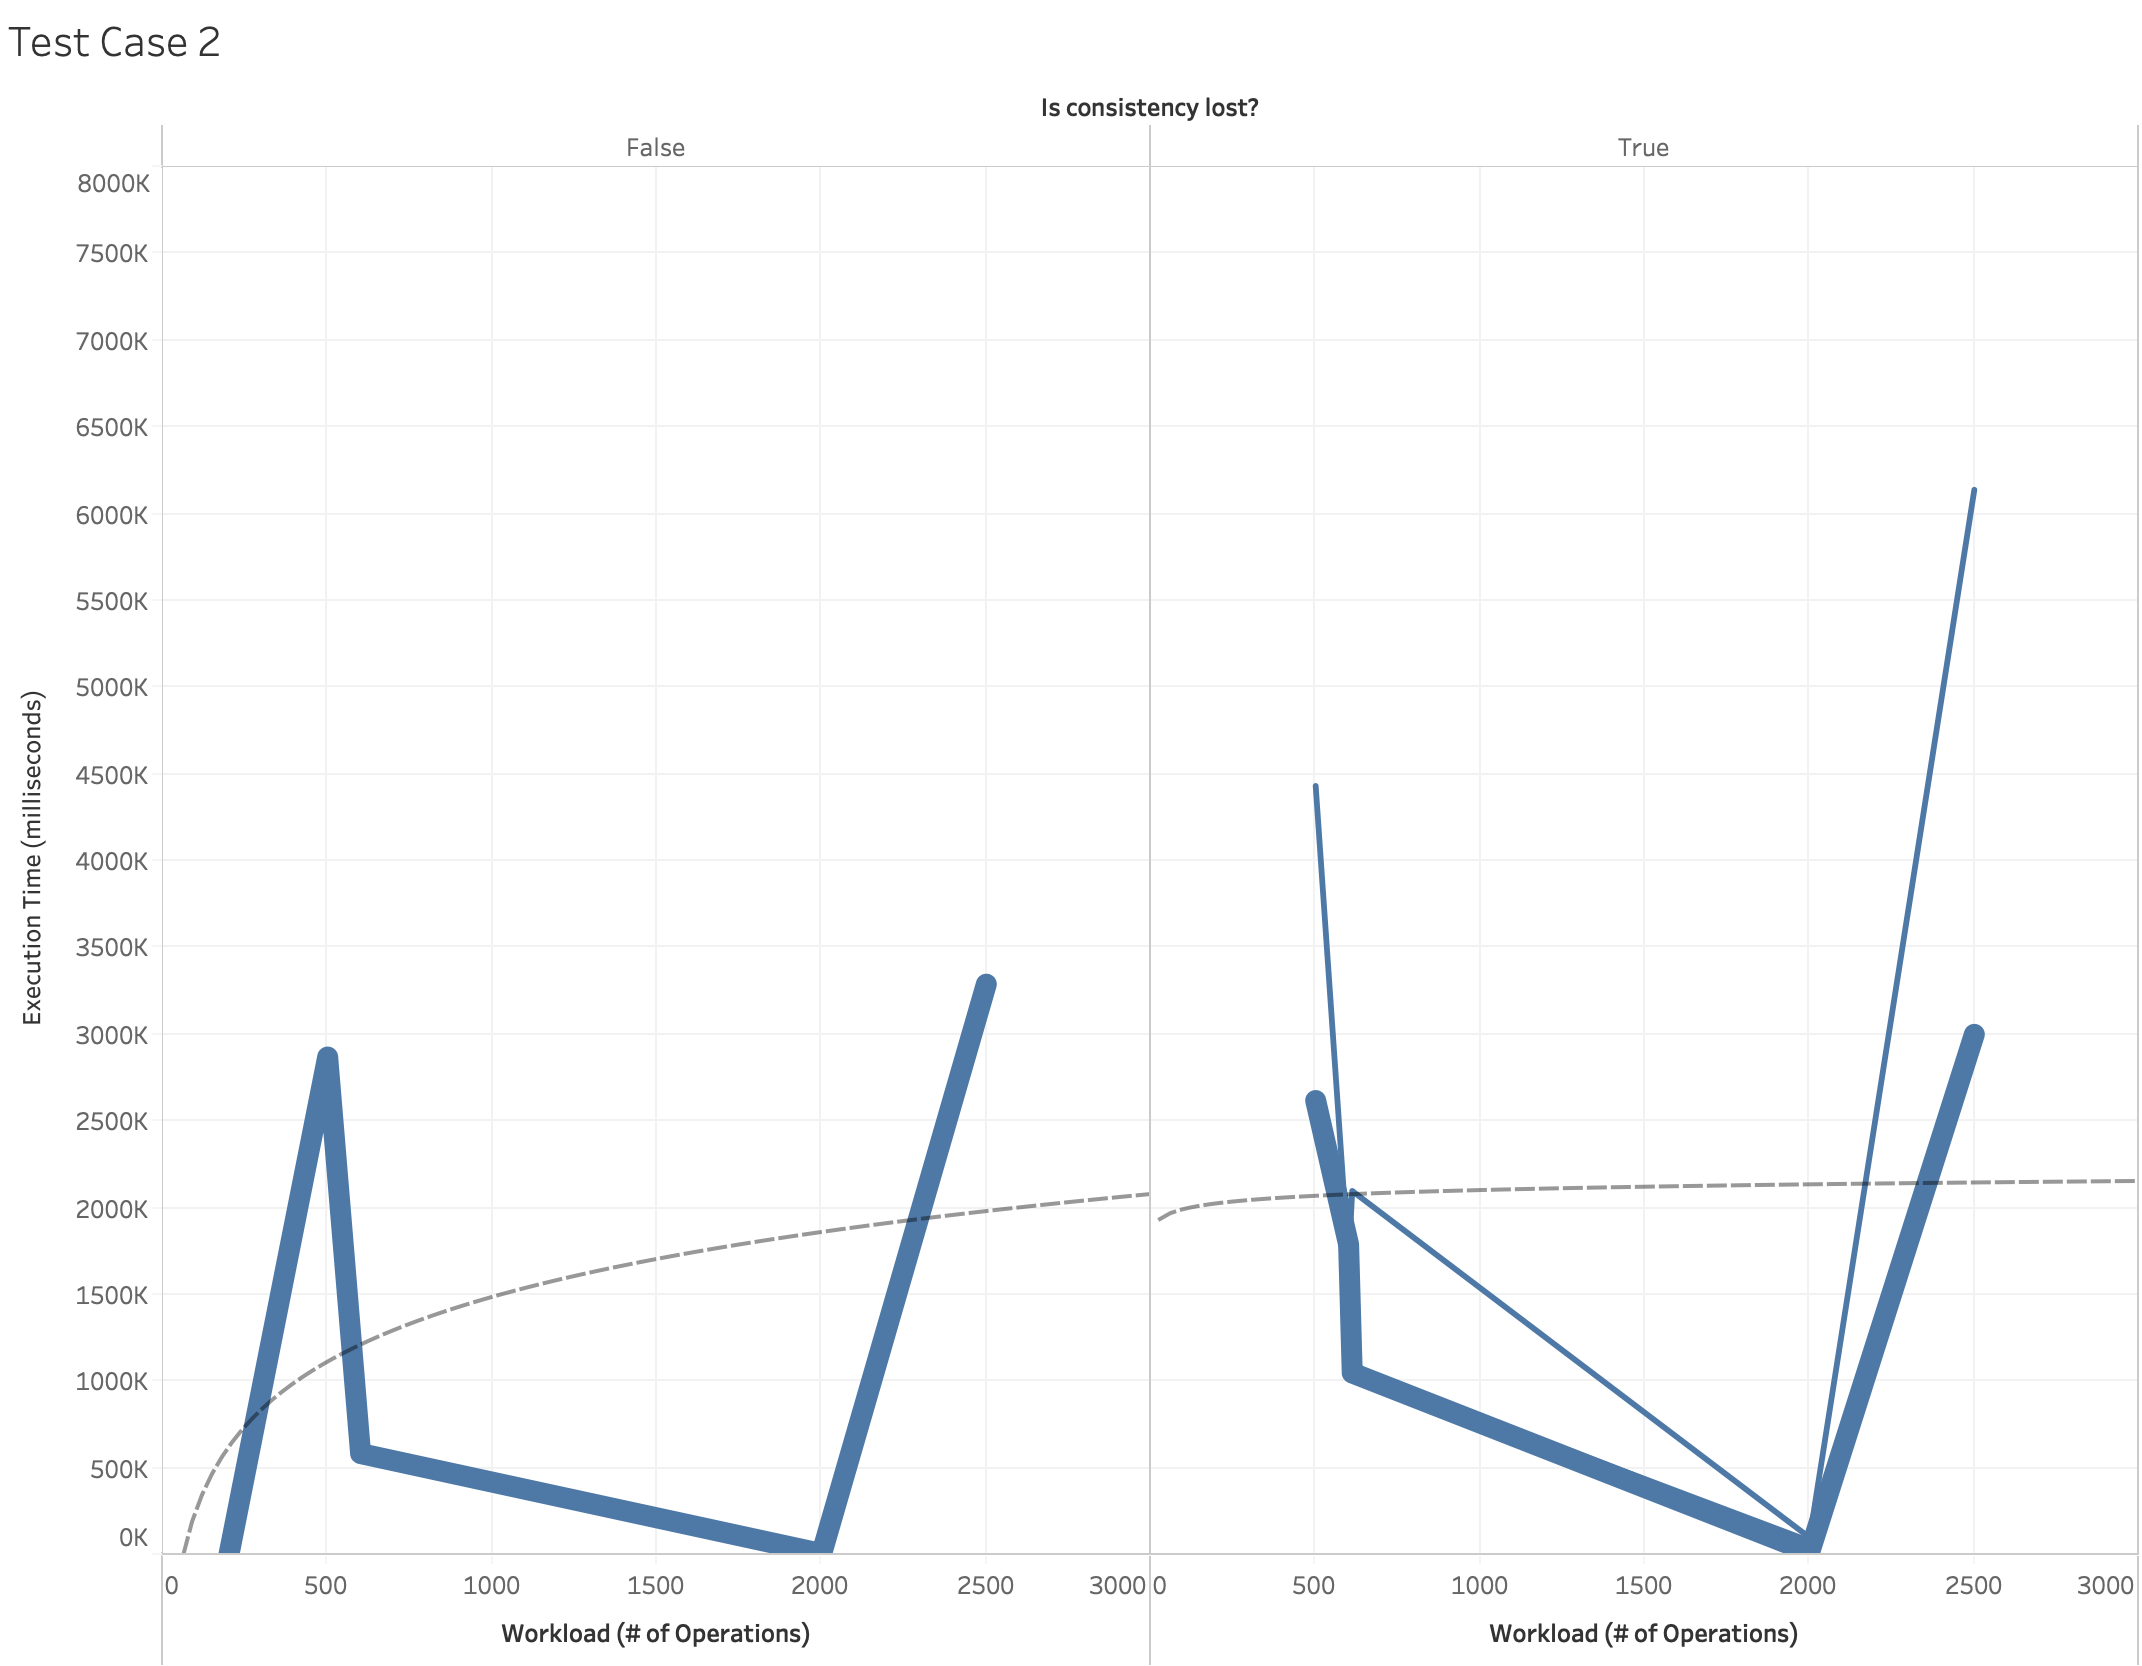
\includegraphics[scale=0.11]{images/TestCase2(WL).png}
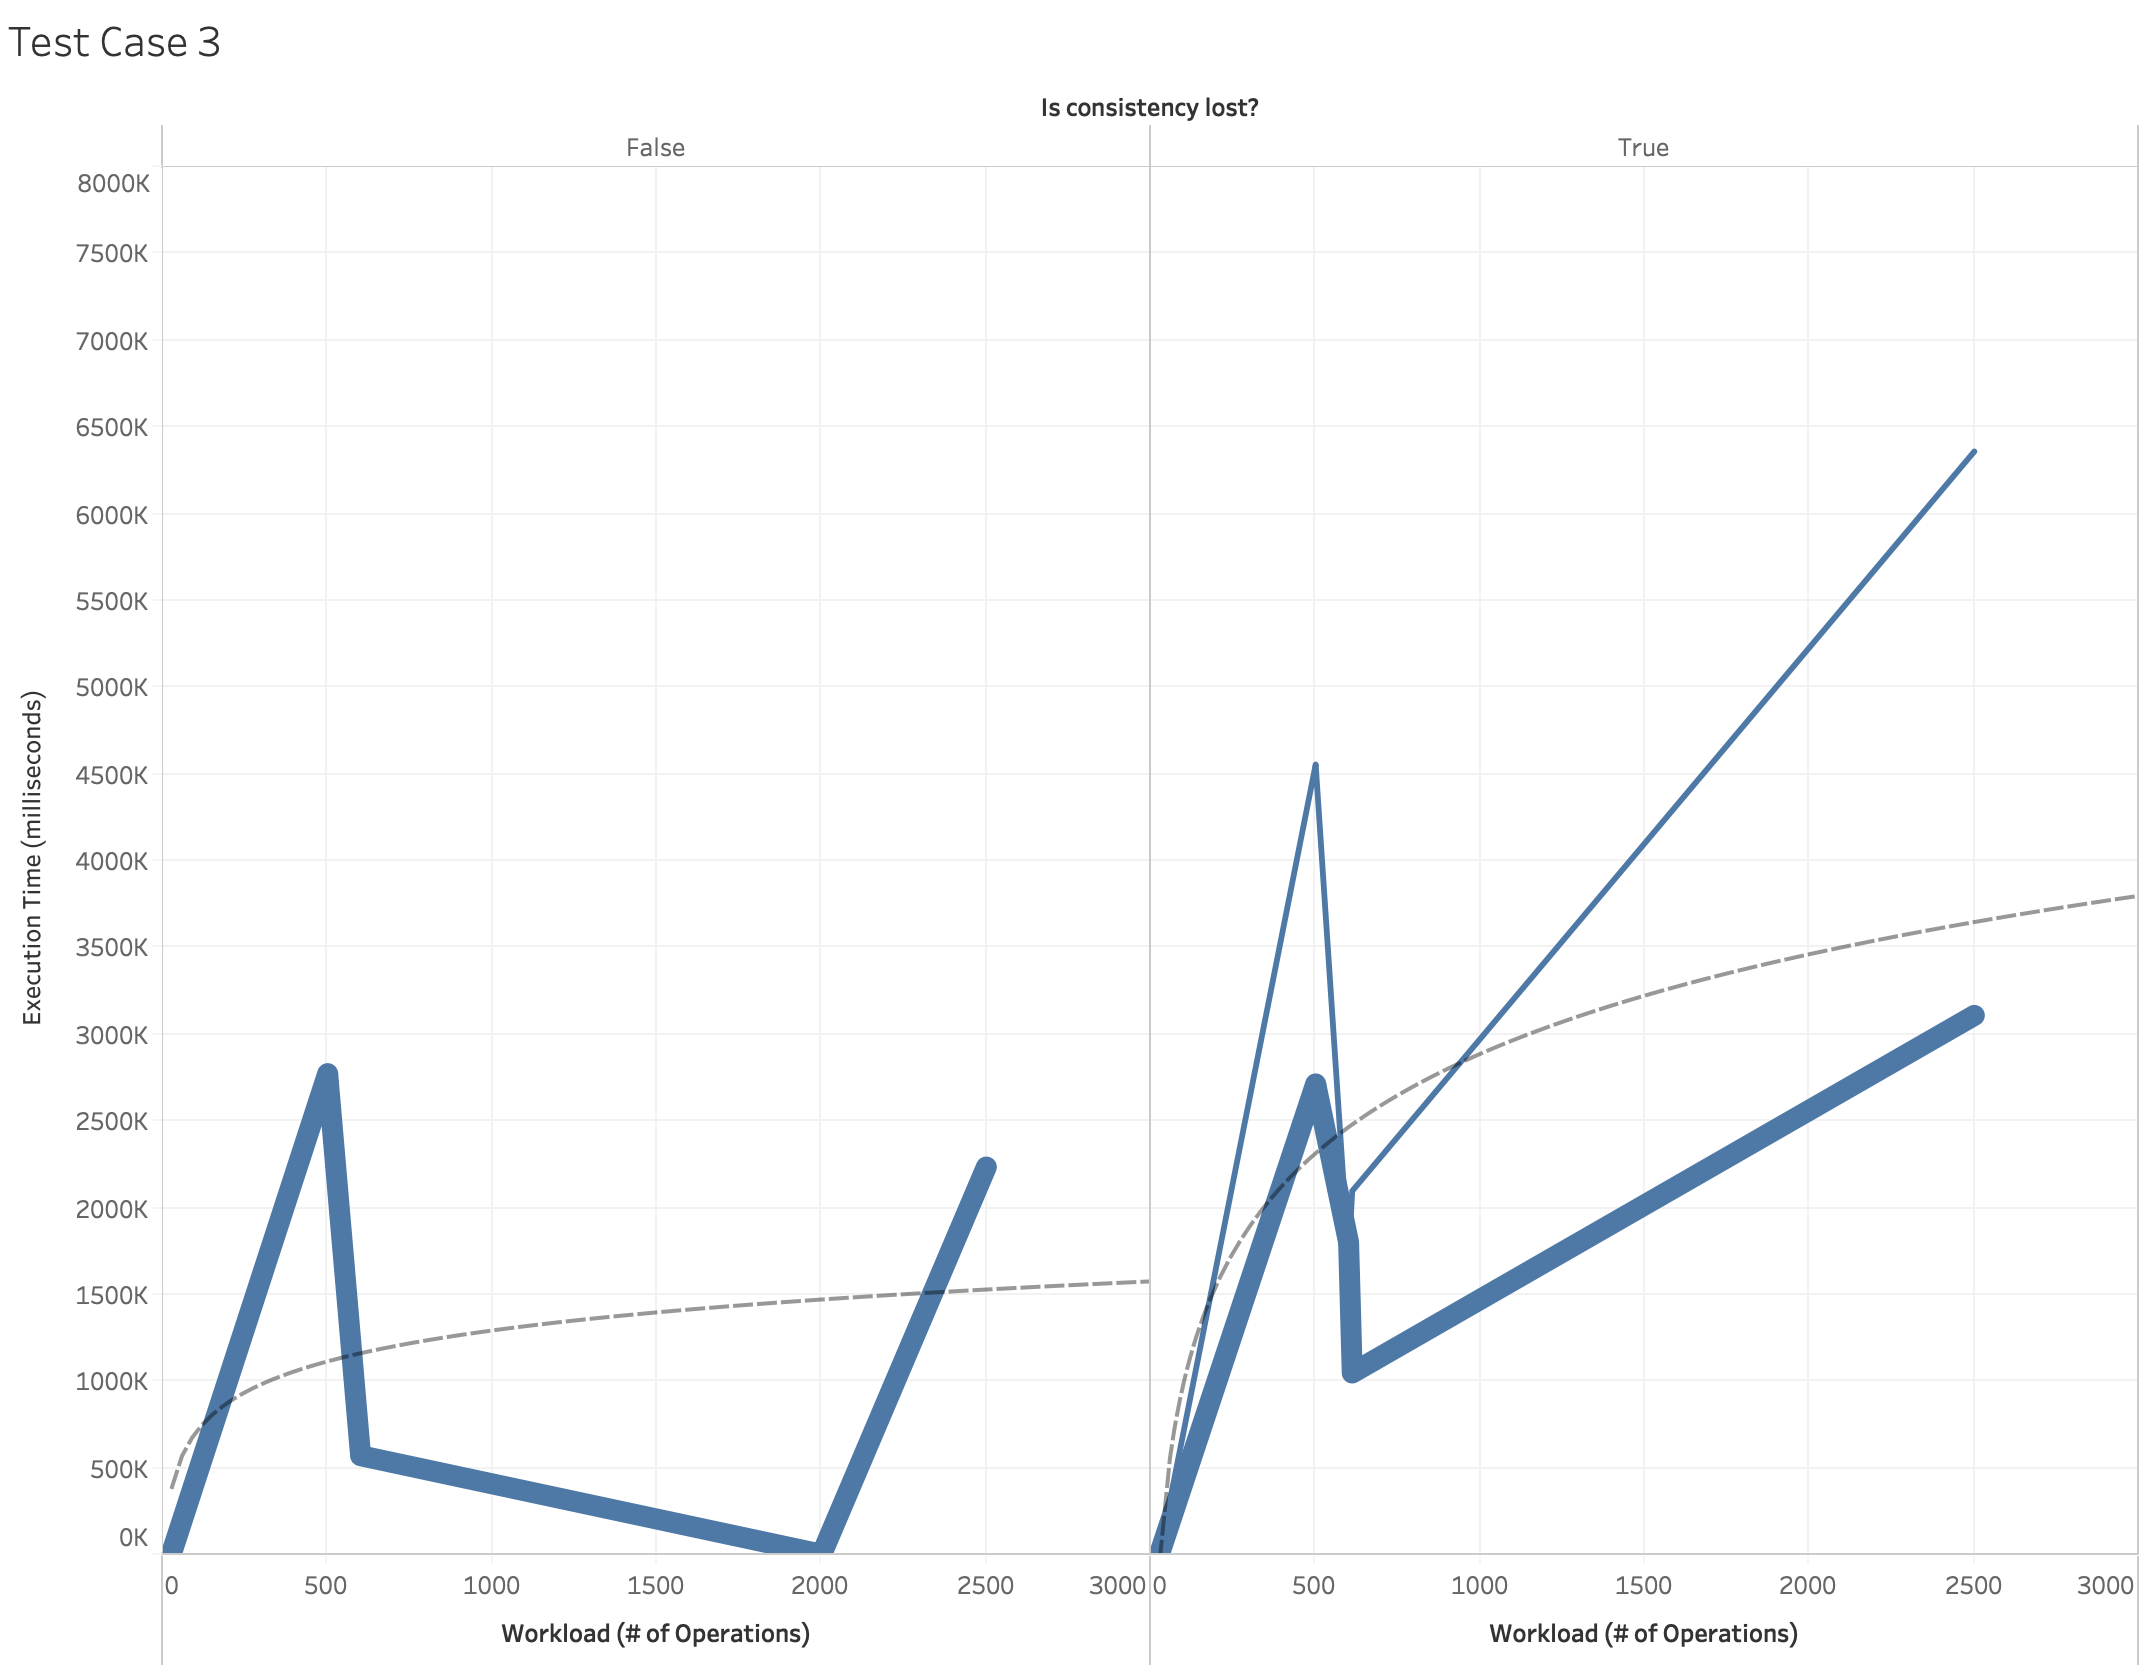
\includegraphics[scale=0.11]{images/TestCase3(WL).png}
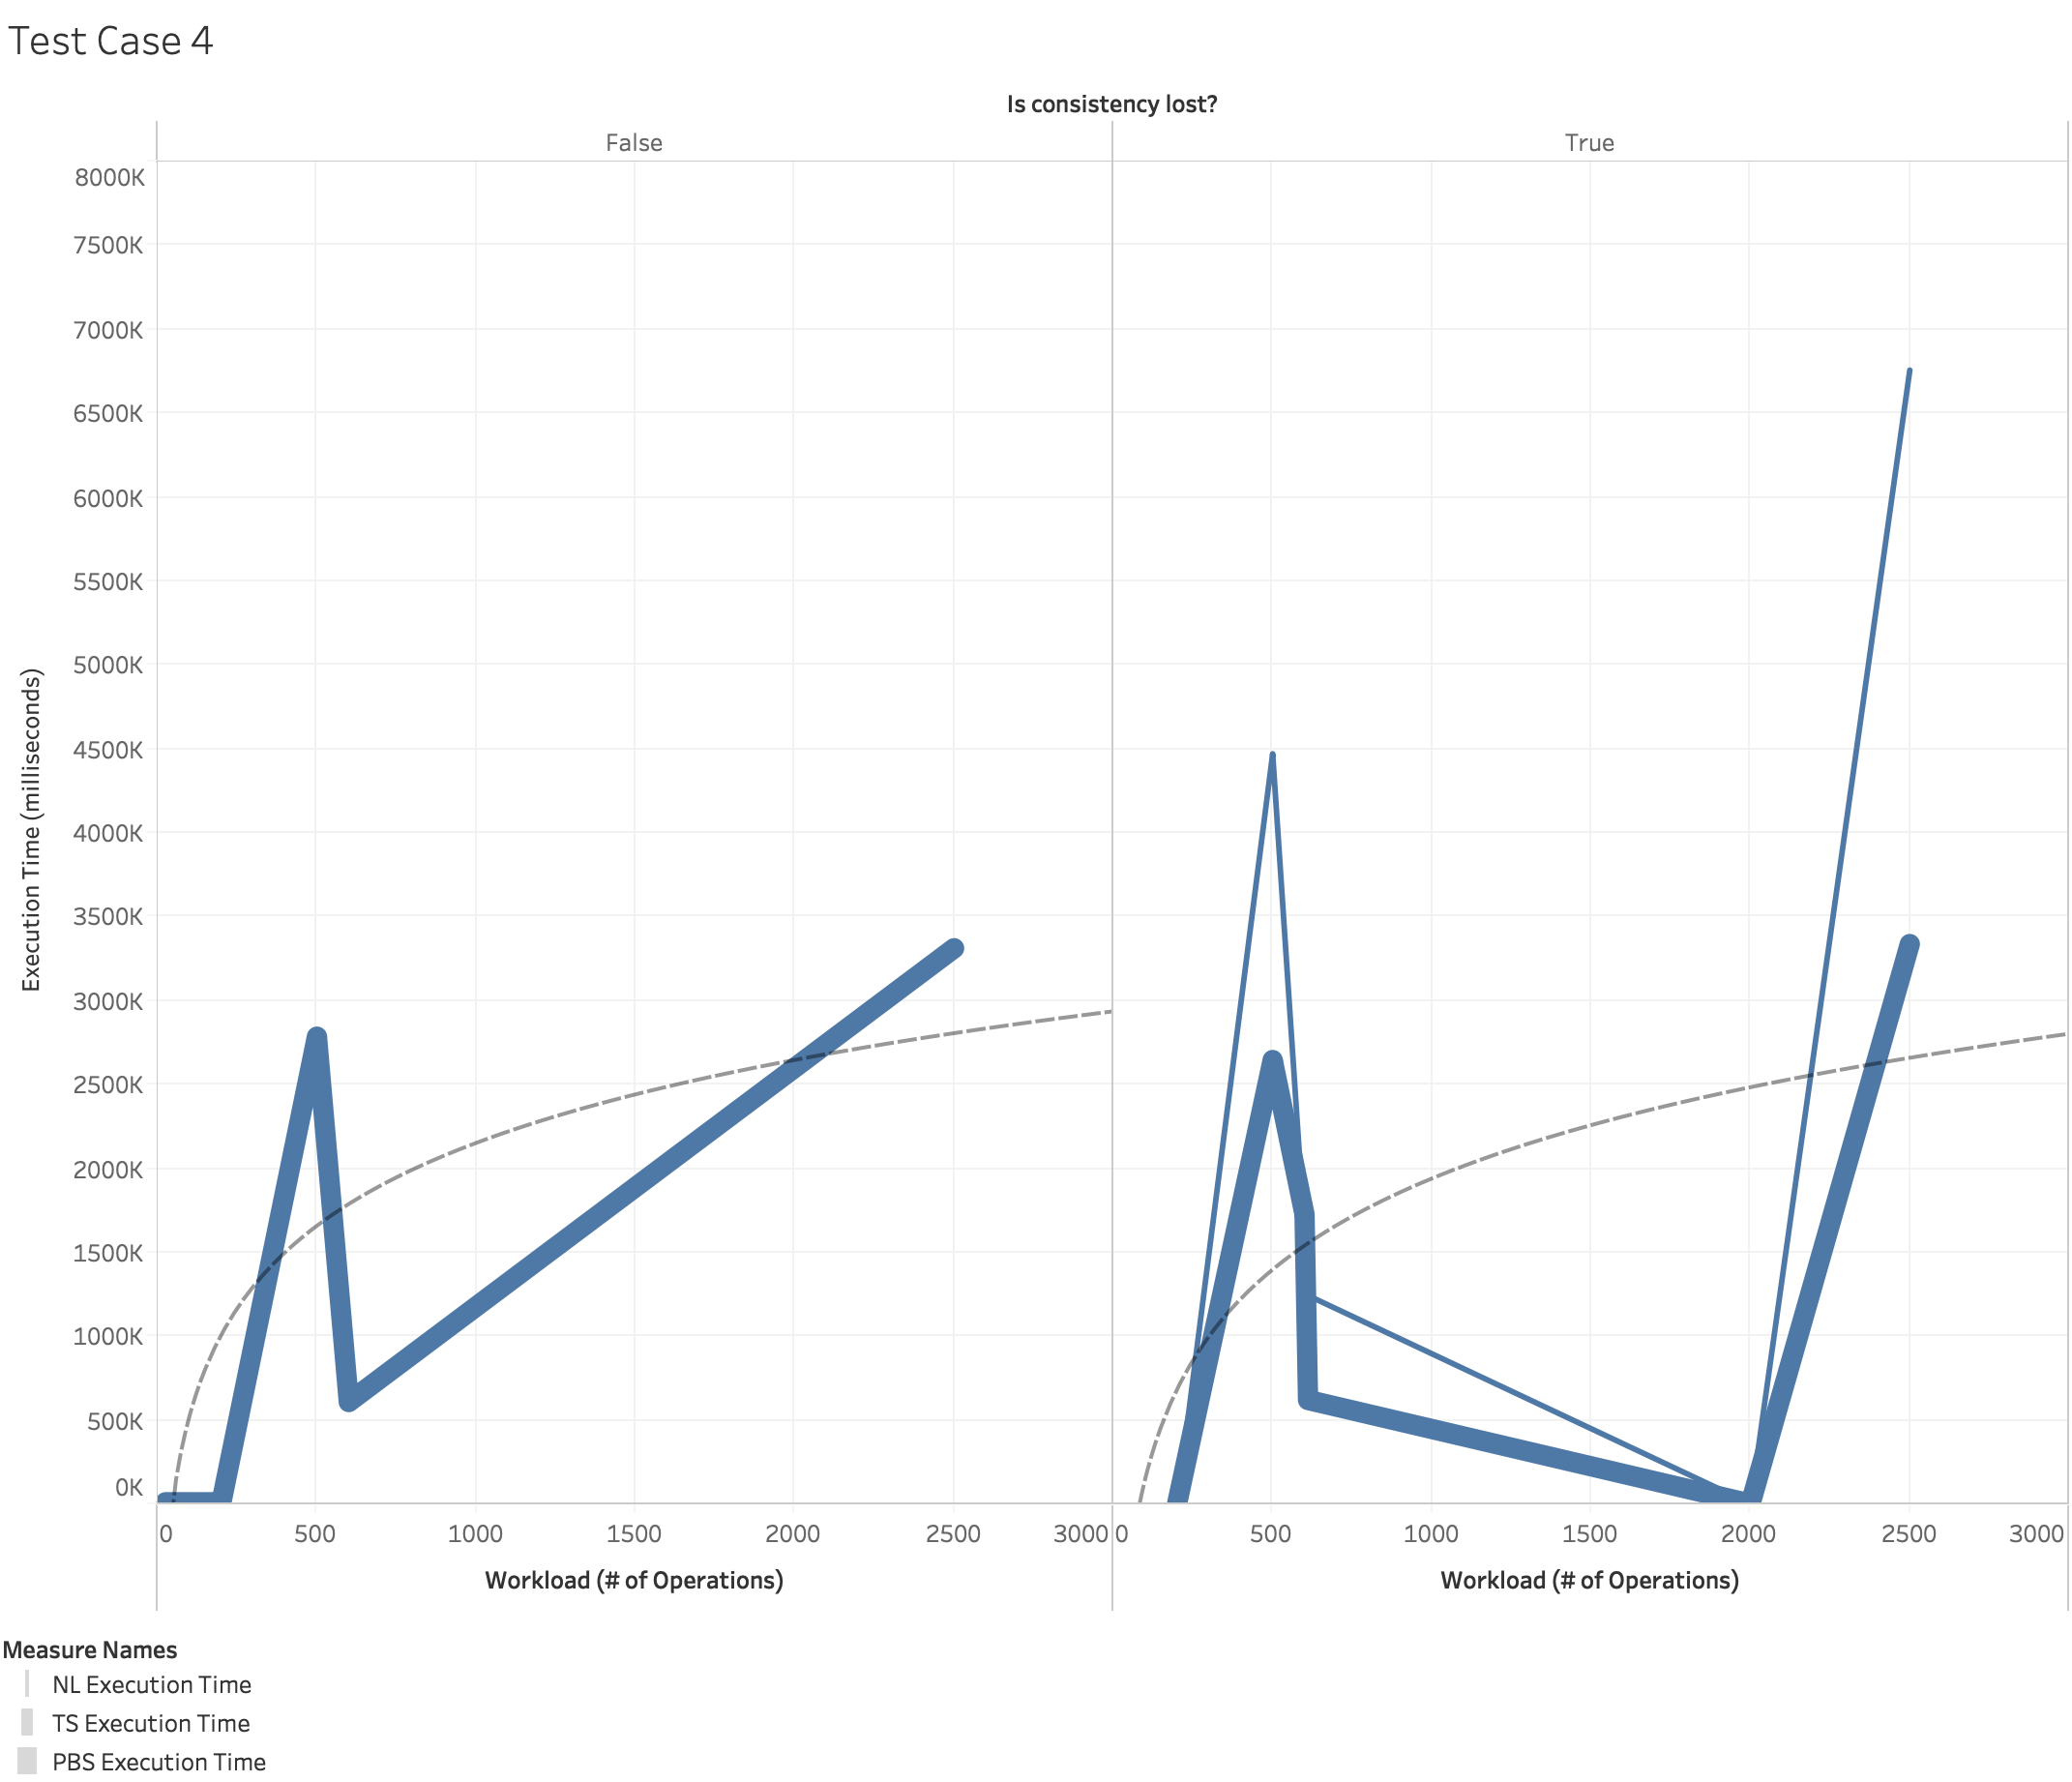
\includegraphics[scale=0.11]{images/TestCase4(WL).png}
\caption{Simulation Results for Test Cases 1-4}
\label{results:test_case_graphs_1_4}
\end{figure}

\begin{figure}
\centering
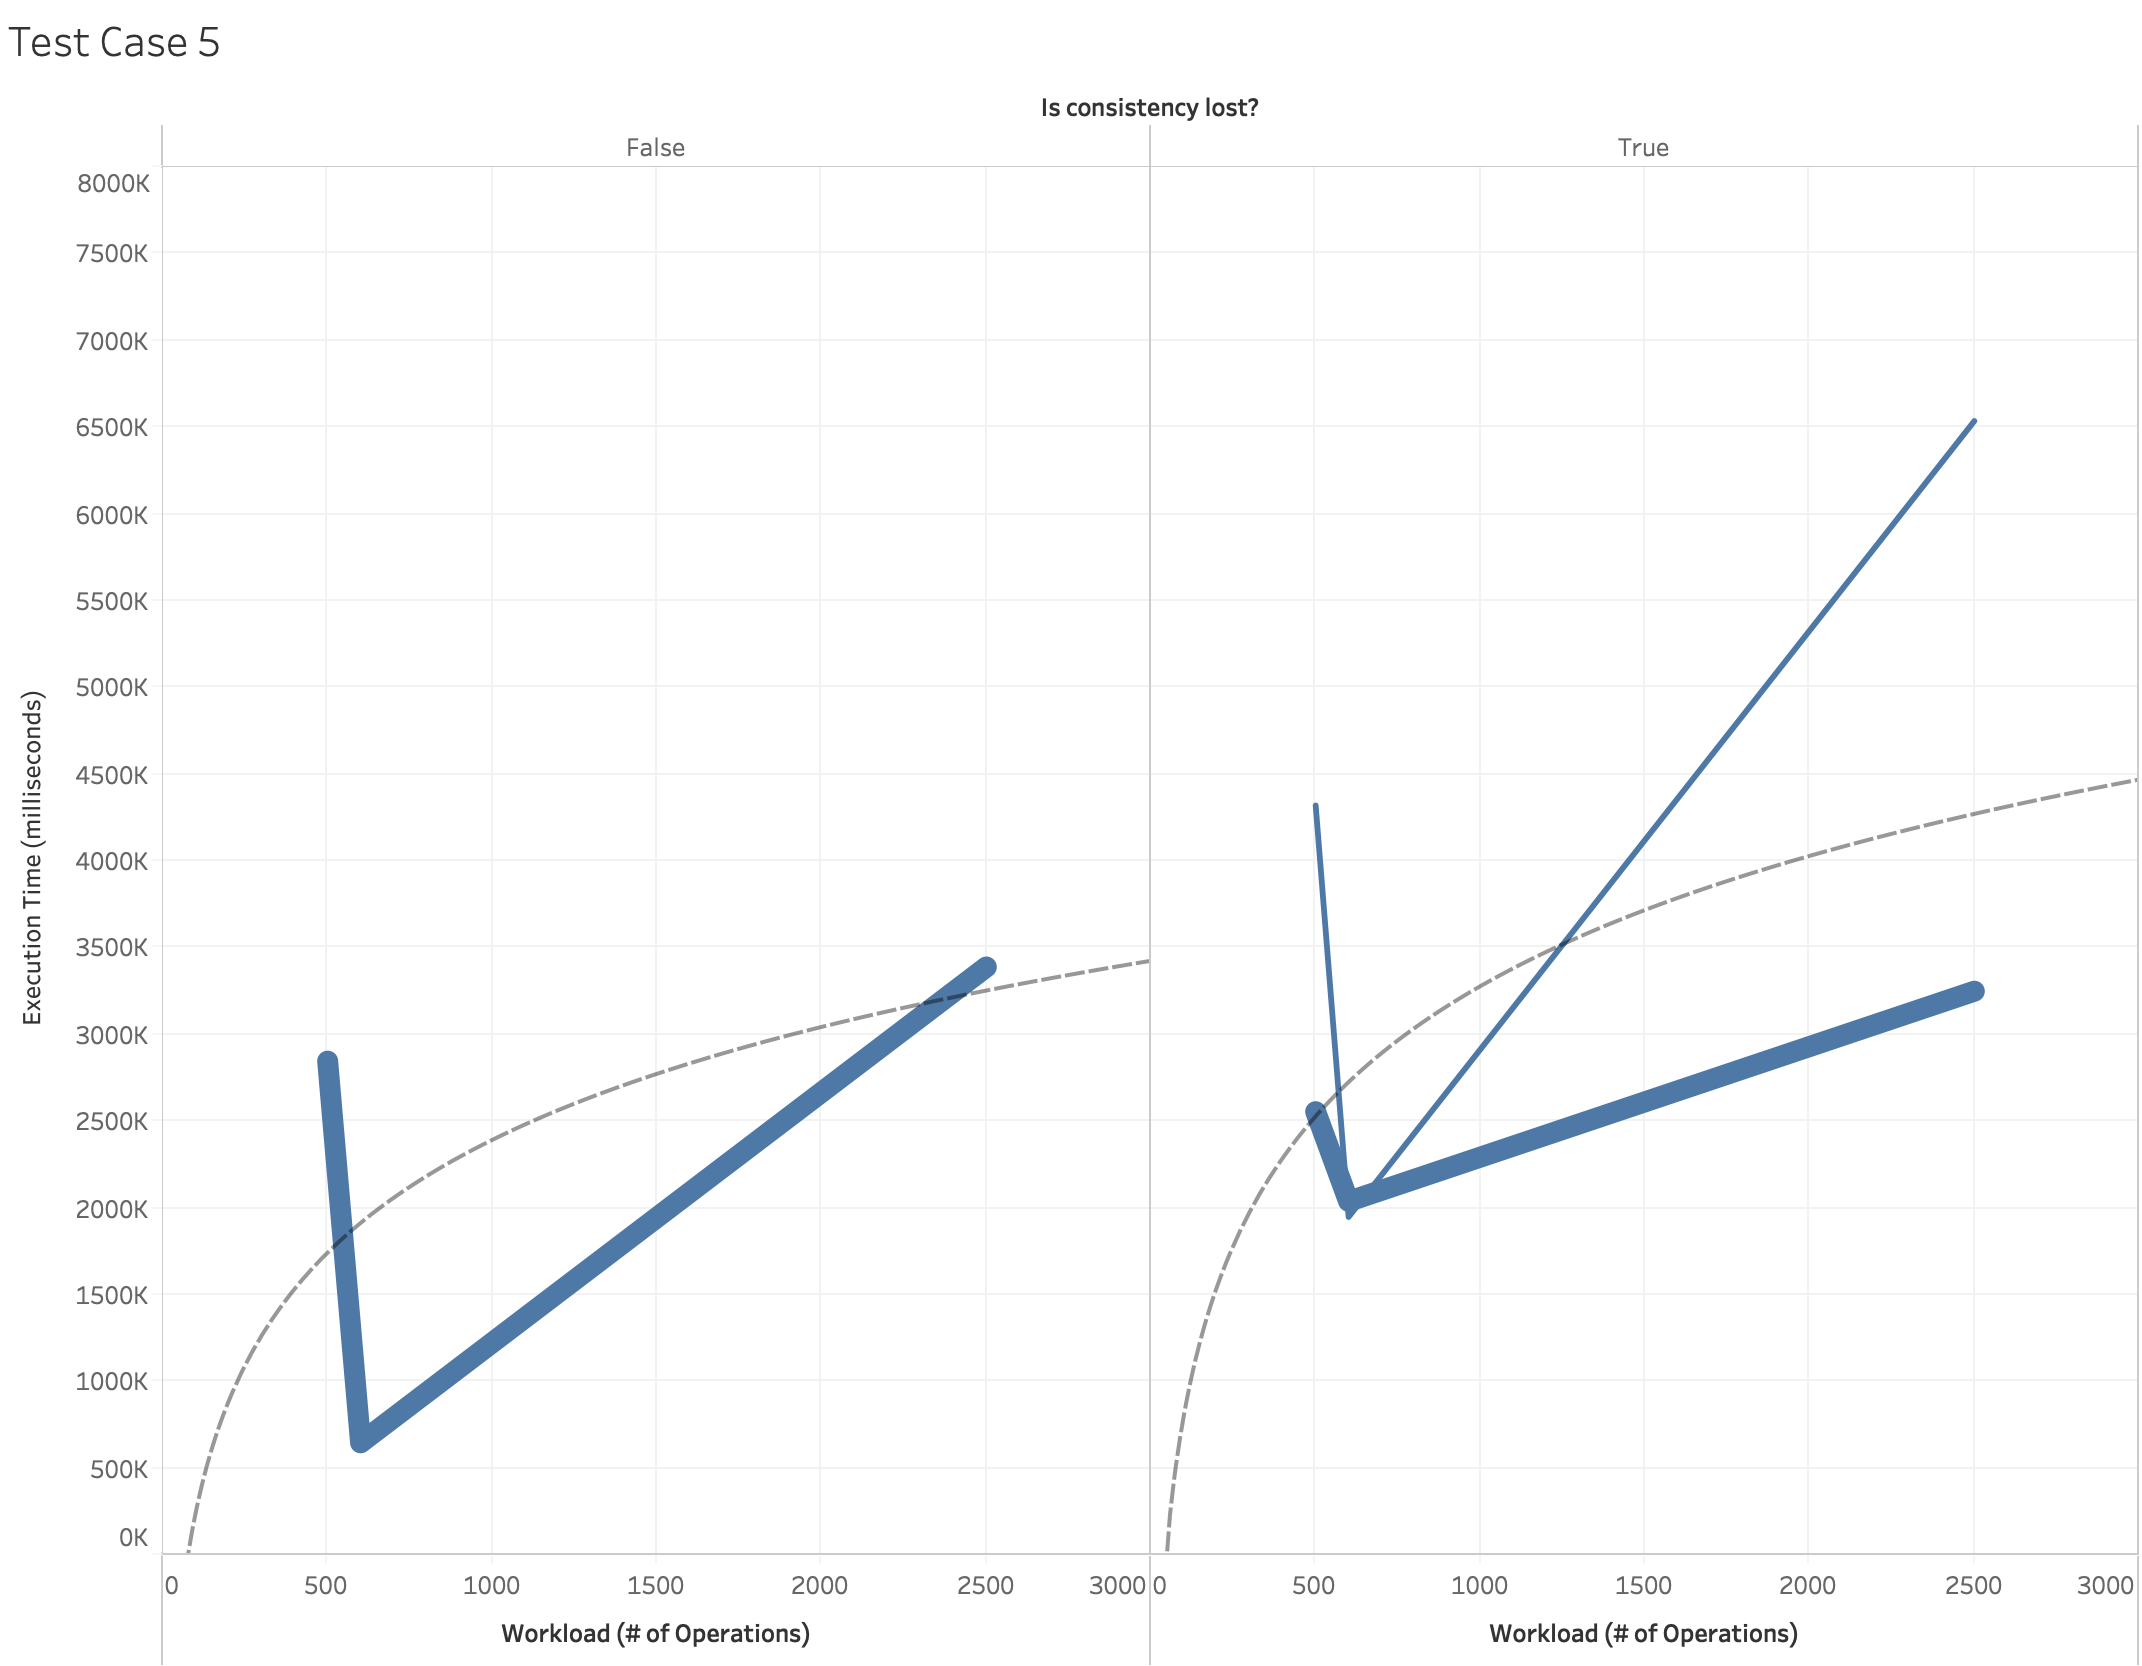
\includegraphics[scale=0.11]{images/TestCase5(WL).png}
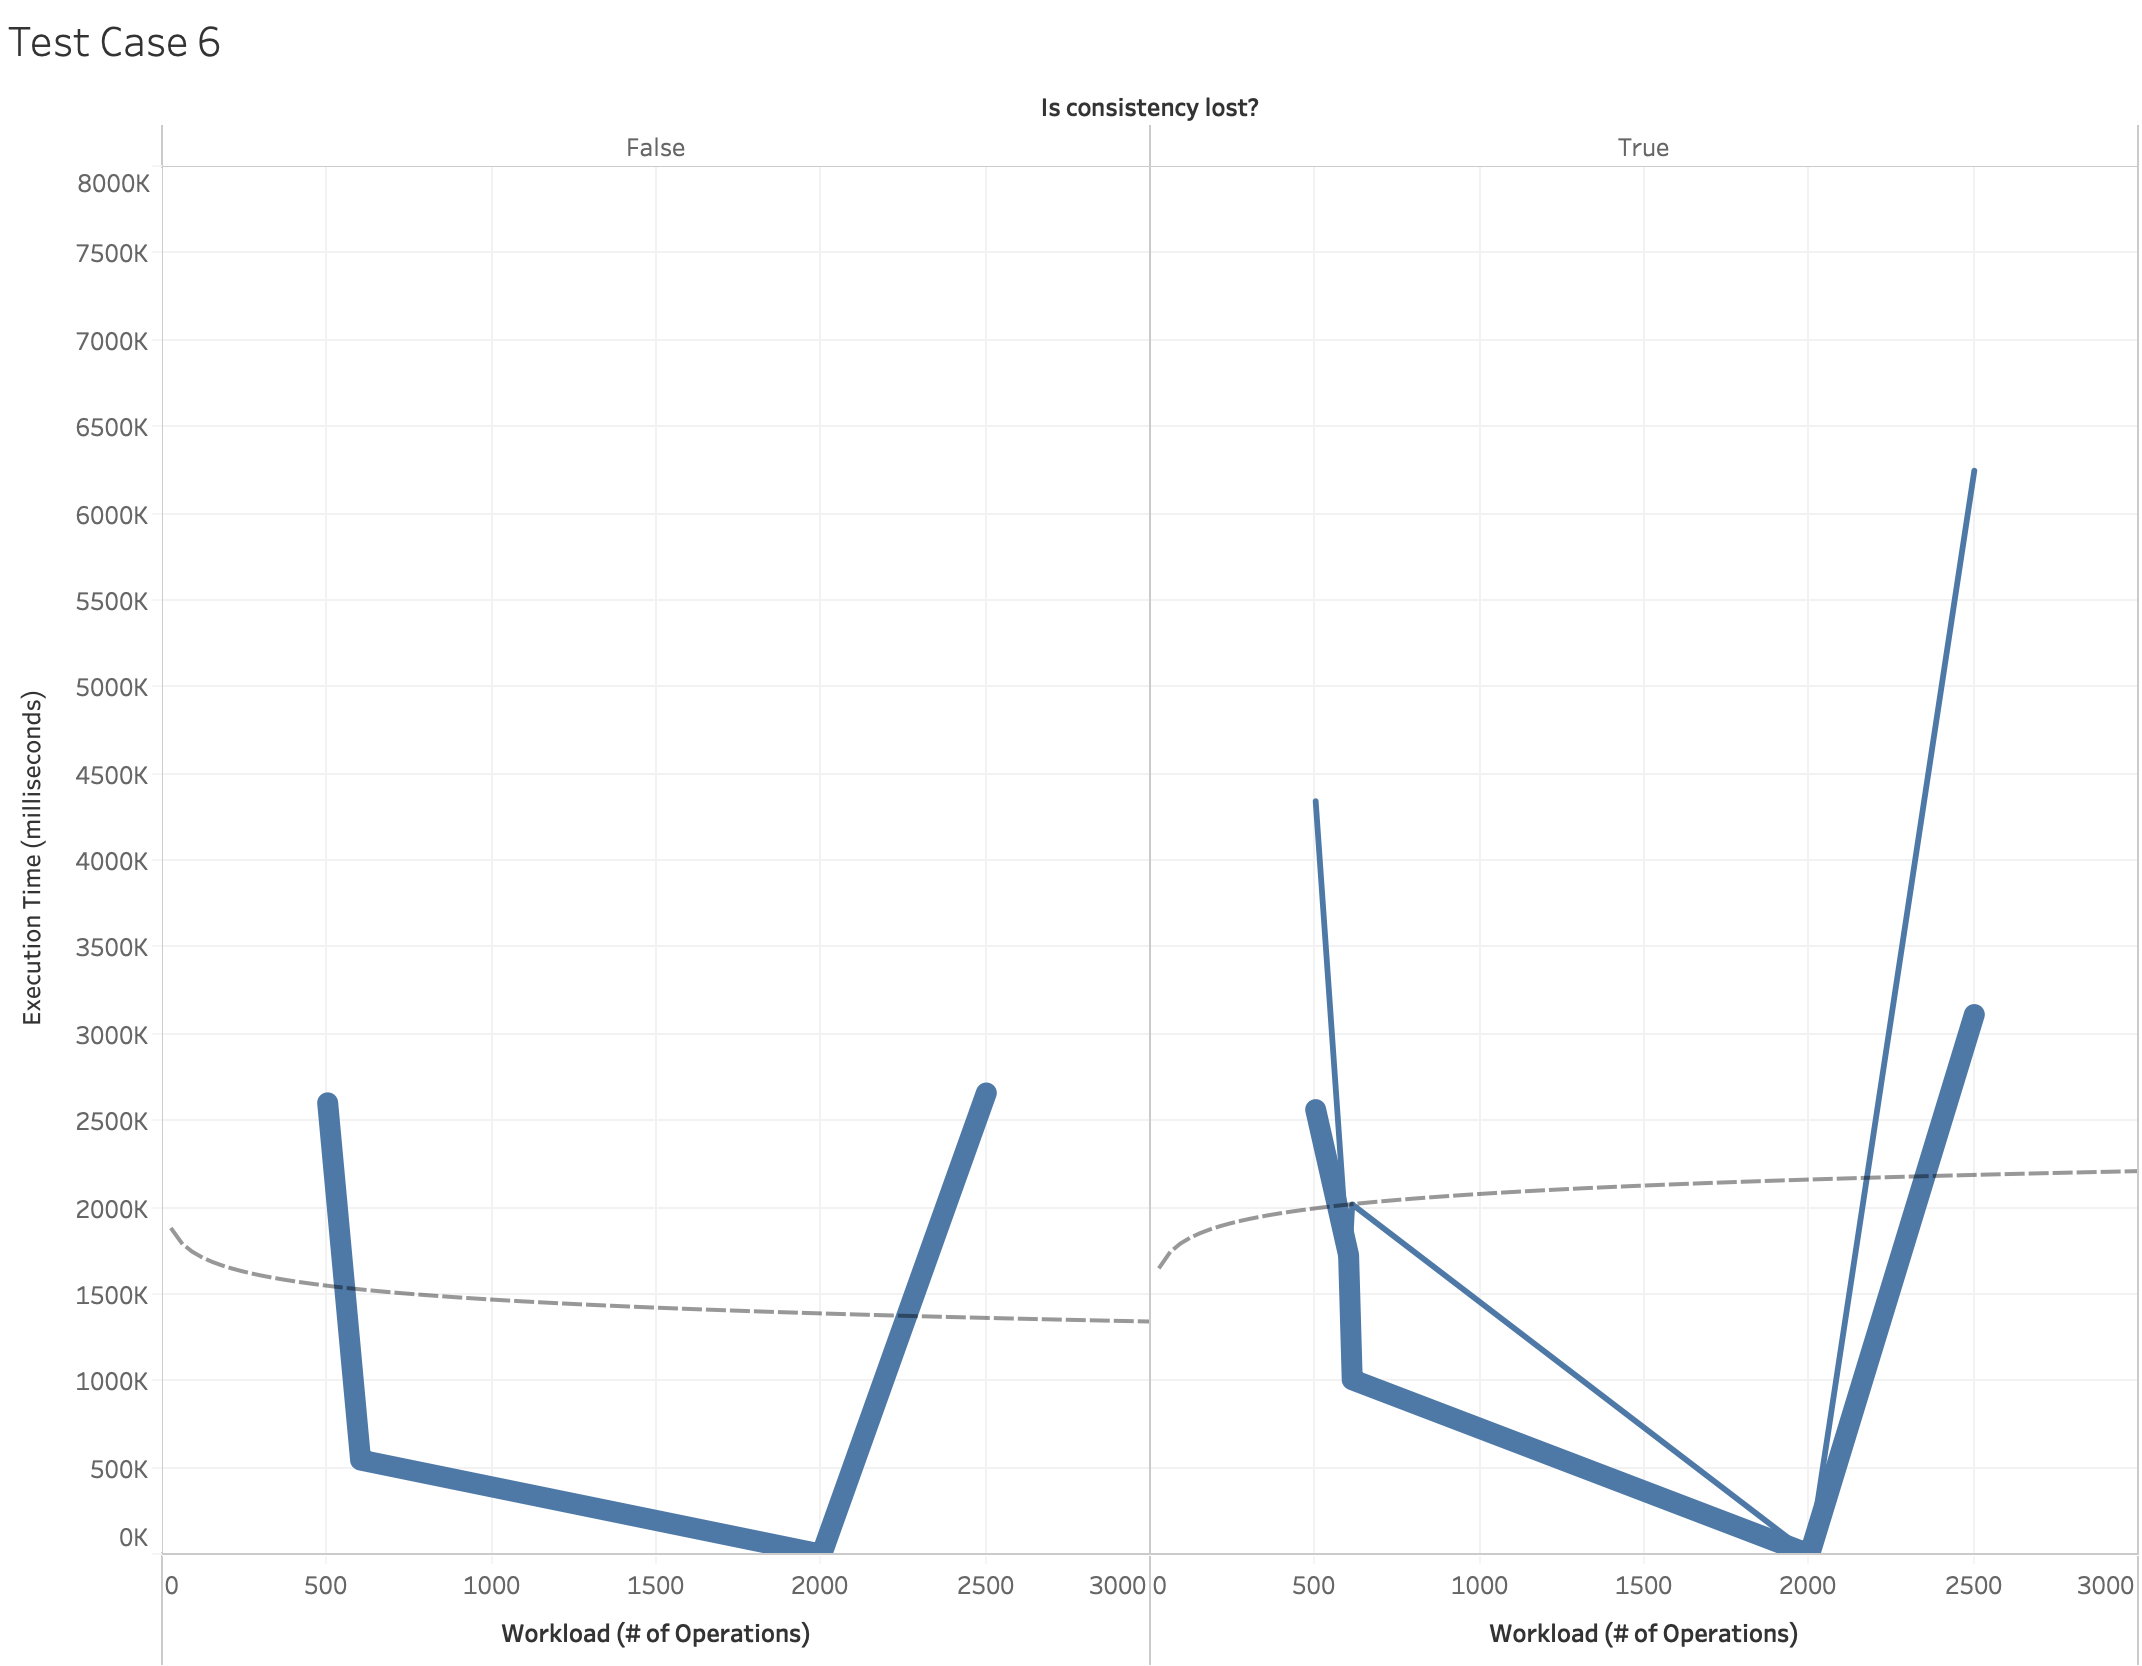
\includegraphics[scale=0.11]{images/TestCase6(WL).png}
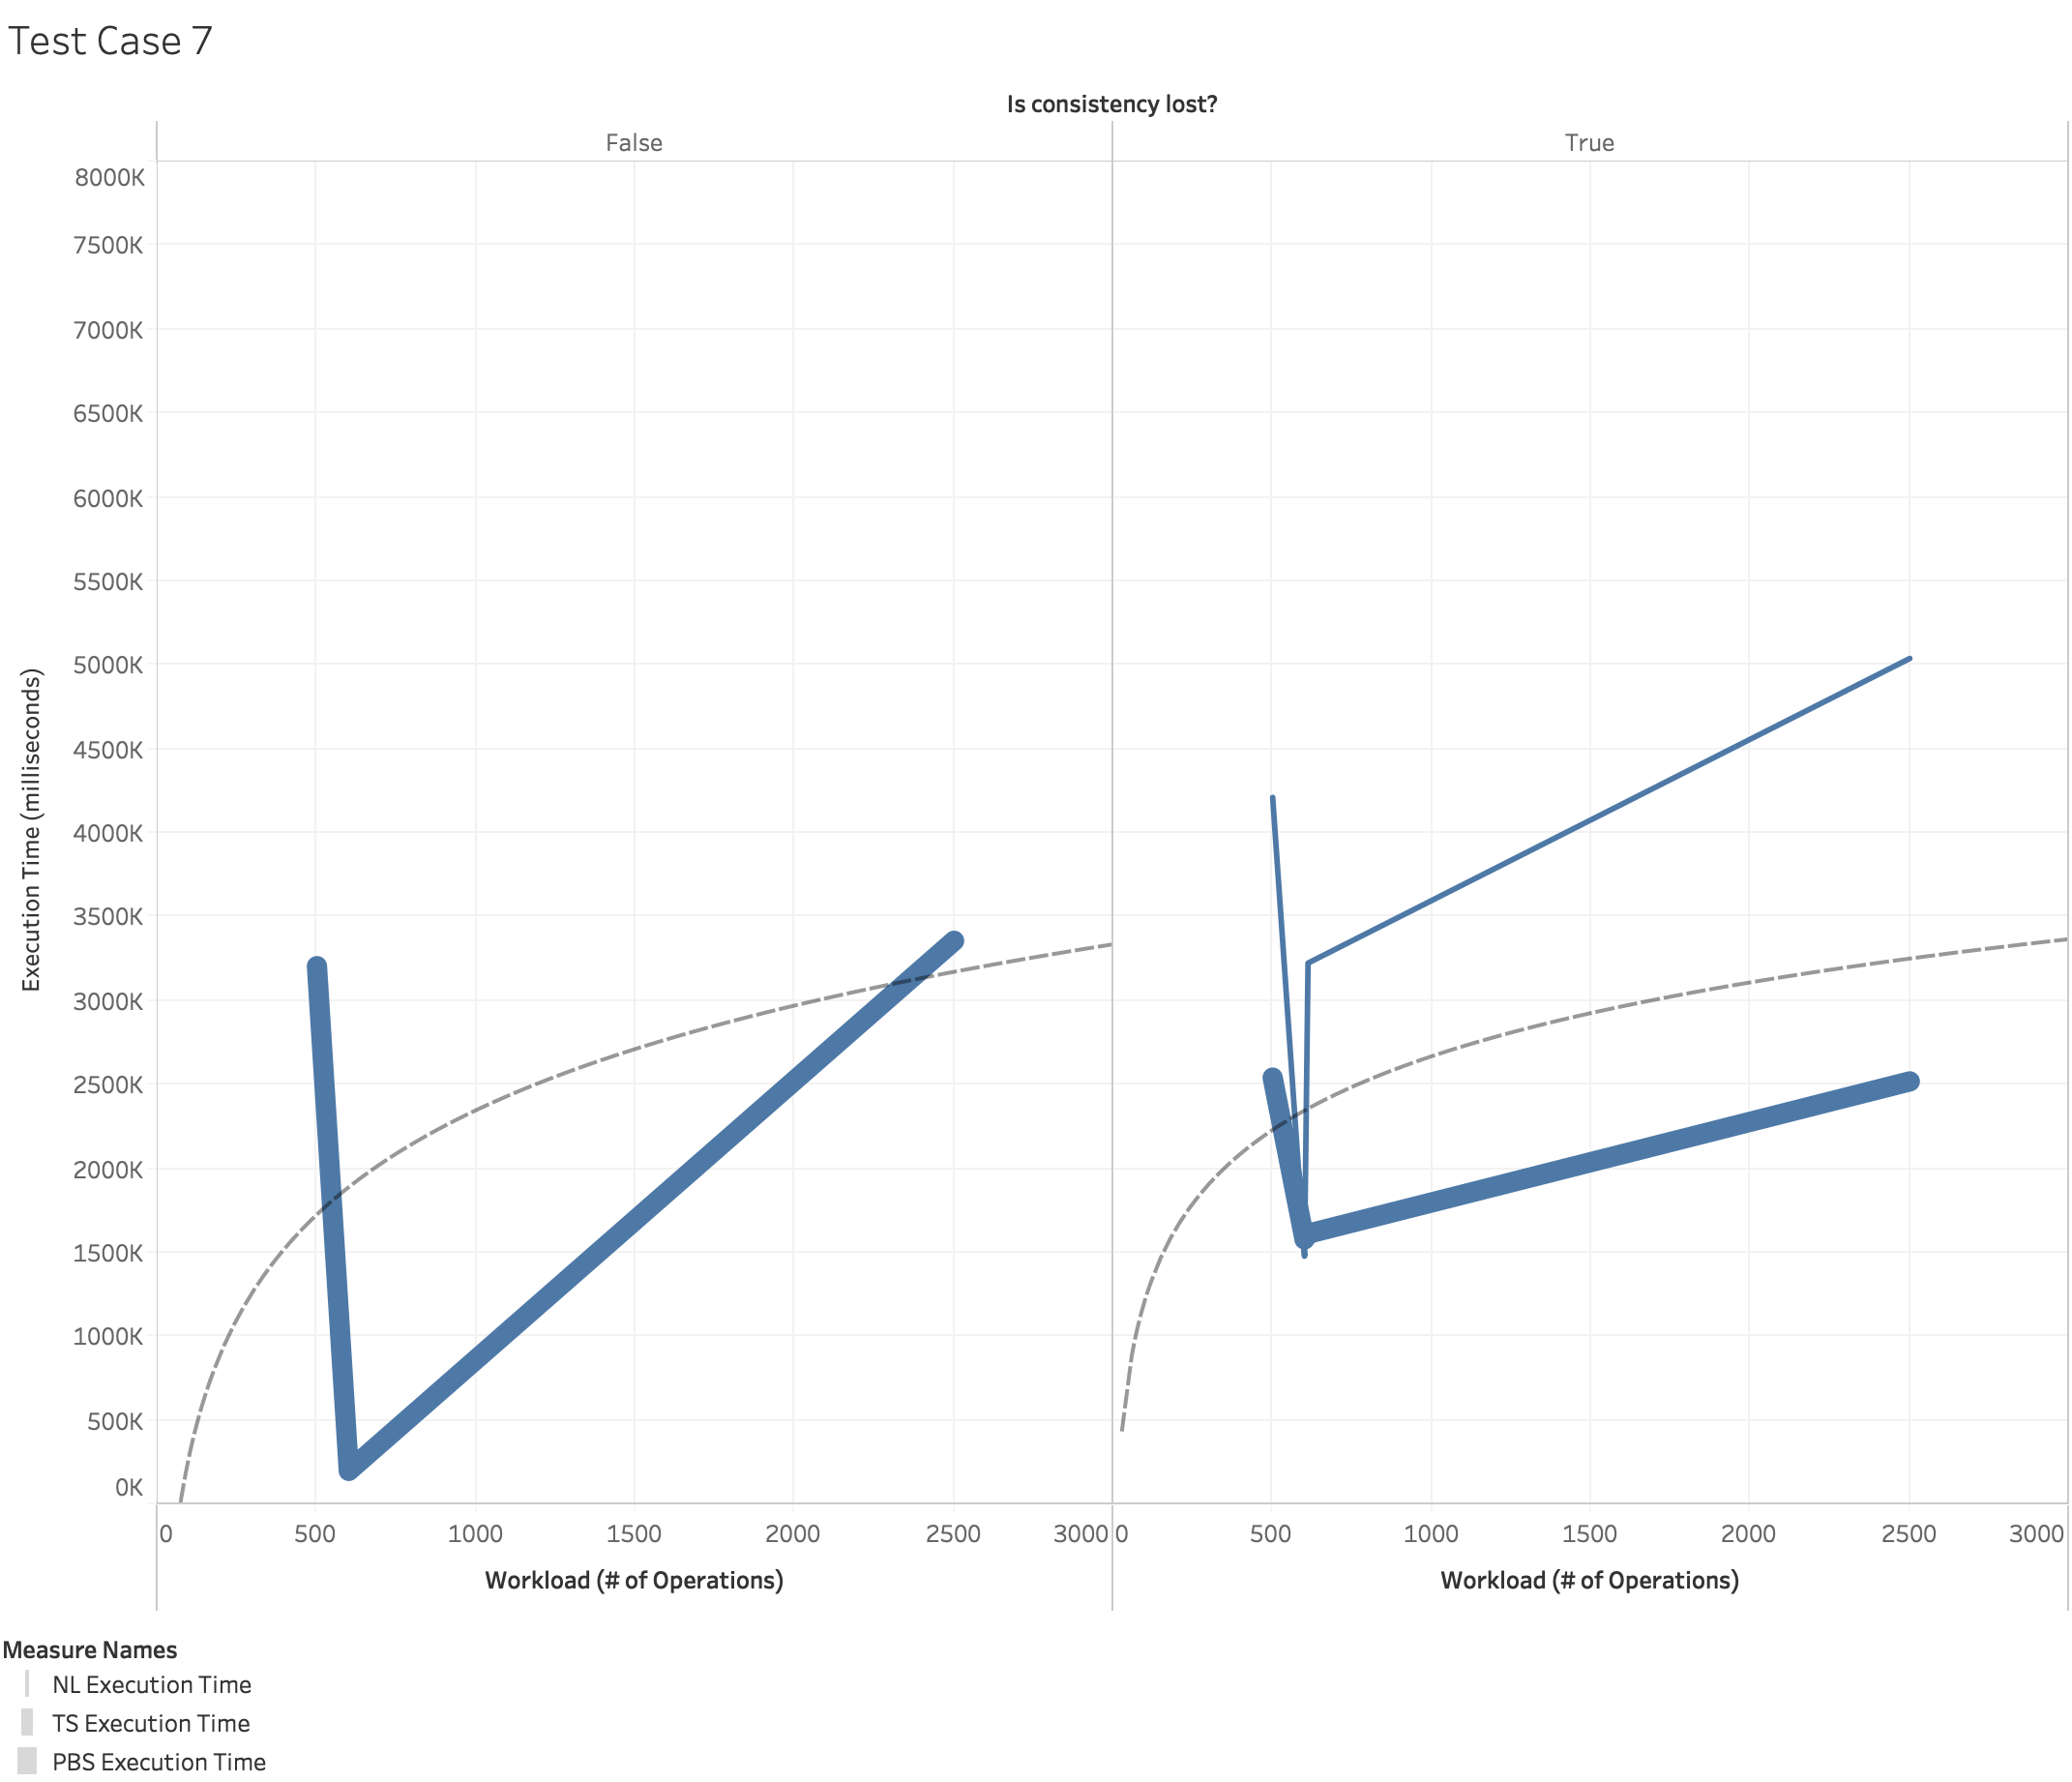
\includegraphics[scale=0.11]{images/TestCase7(WL).png}
\caption{Simulation Results for Test Cases 5-7}
\label{results:test_case_graphs_5_7}
\end{figure}

\begin{figure}
\centering
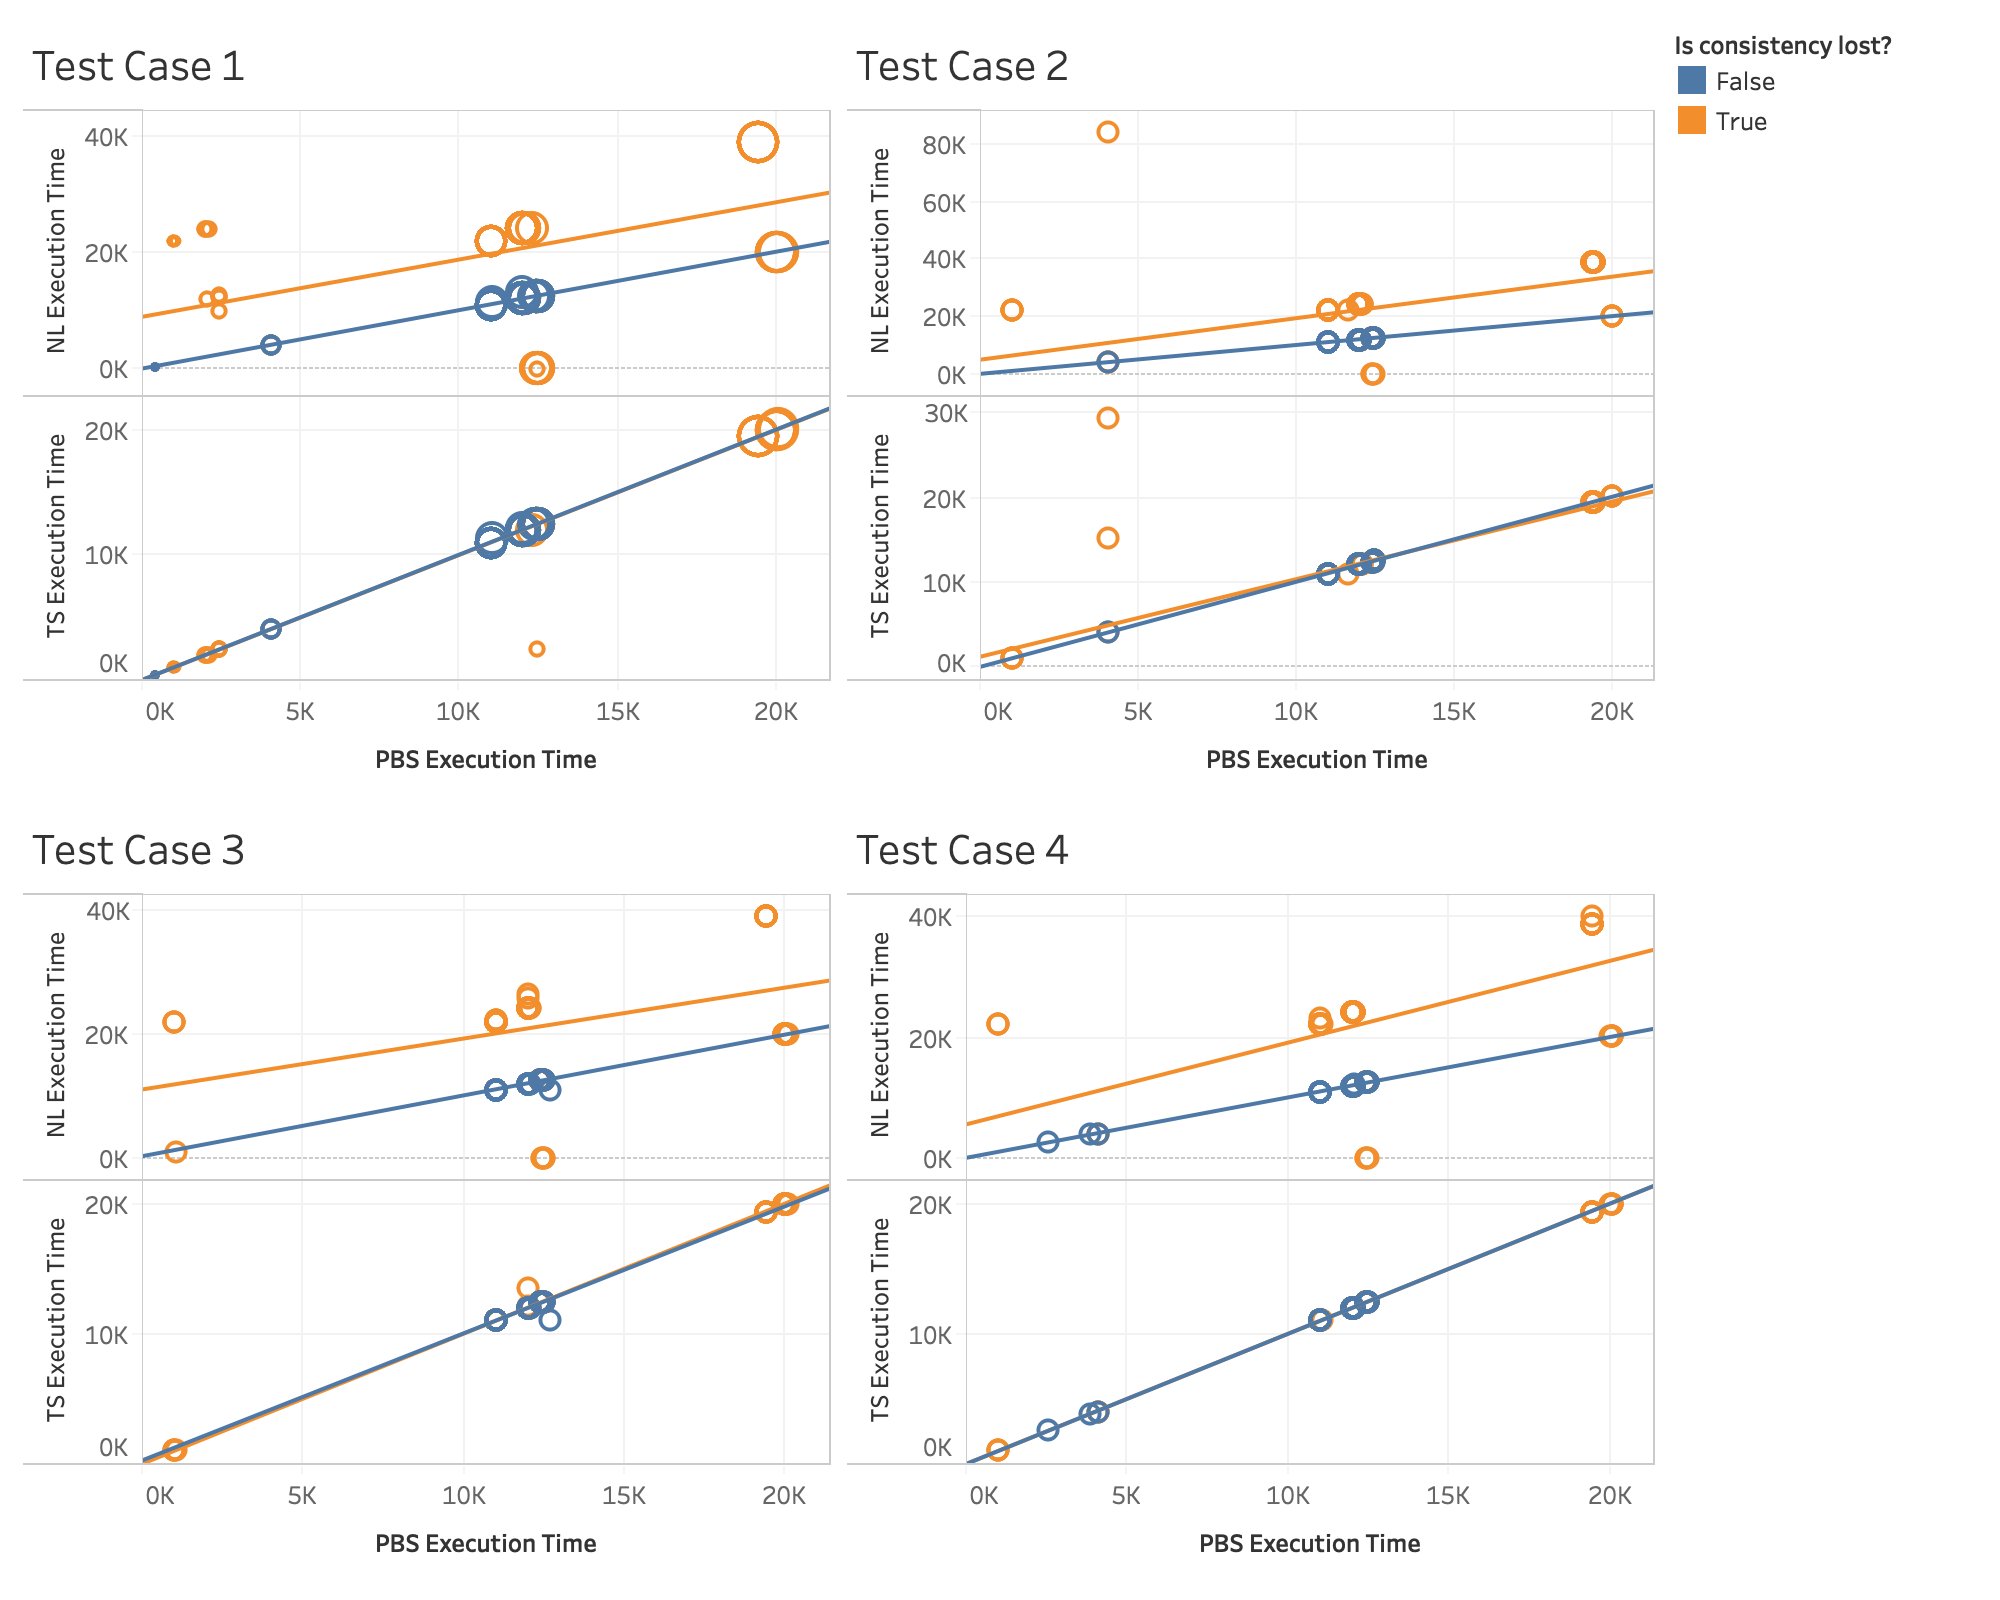
\includegraphics[scale=0.13]{images/Dashboard1_TL.png}
\caption{Consistency Lost/Kept for Test Cases 1-4}
\label{results:consistency_test_case_graphs_1_4}
\end{figure}

\begin{figure}
\centering
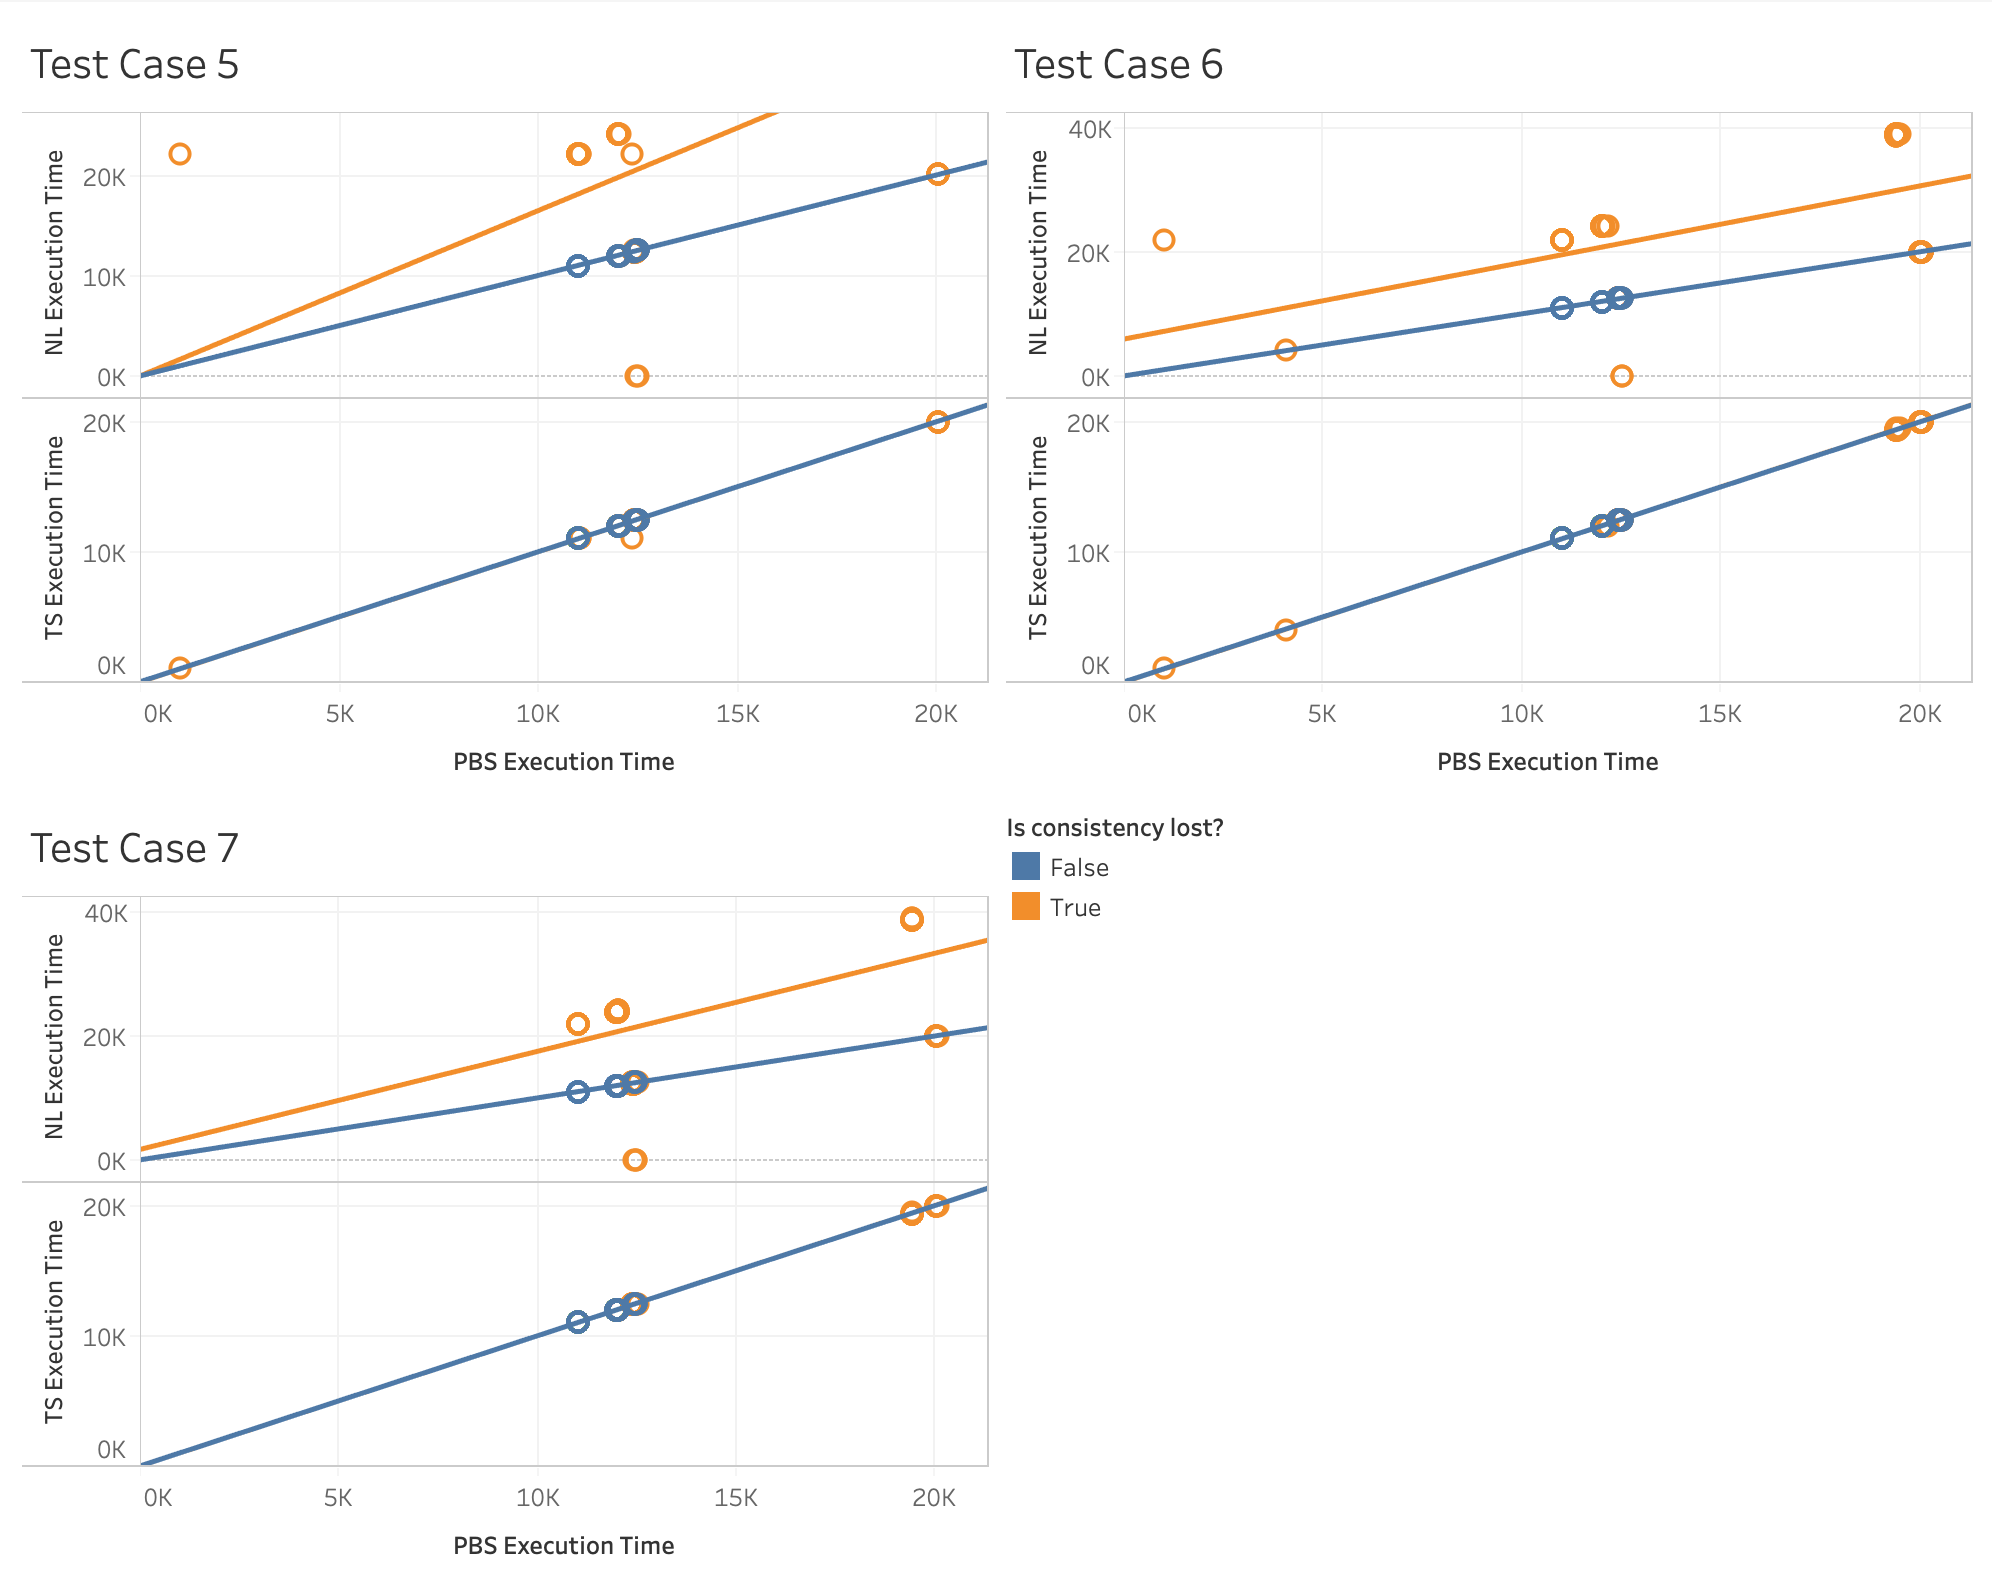
\includegraphics[scale=0.21]{images/Dashboard2_TL.png}
\caption{Consistency Lost/Kept for Test Cases 5-7}
\label{results:consistency_test_case_graphs_5_7}
\end{figure}